\label{sec:introduction}
\section{Introduction}

The word psychology literally means, ”the study of the soul”. This gives the idea of the vastity of the field of study of psychological sciences: the mind.
Studying the mind is quite a complex task because of the immateriality and unobservability of the subject of study.
To circumvent this limitation psychologists have developed different research techniques that aim to analyze constructs not directly observable.
Amongst these tools, psychology makes a significant use of tests to perform its analysis (like in \cite{Cohen-1992}).\\
\\
A psychological test is an instrument created and designed to measure psychological constructs, modeled through so called latent variables.
Psychological tests are typically, but not necessarily, a series of tasks or problems that the respondent has to solve.
Many different test techniques have been developed over time, one of the most structured and quantitative is represented by personality inventories
(with the different approaches compared in \cite{Burisch-1984}) or structured multiple-choiche tests.
In these tests, the subject is requested to go through a series of questions and provide answers choosing between different options presented.
These choices could be structured on different scales (one of the most commonly used scales is the \cite{Likert-1932} scale).\\
\\
The possible fields of application of psychological studies are very numerous and broad.
Together with the study of singular cases and the generalization of mental constructs, psychology very often refers to the sociological world.
Social psychology (\cite{Smith-2006}) is defined as the scientific study of how people's thoughts, feelings, and behaviors are influenced by the actual, imagined,
or implied presence of others.
Social psychologists typically work to explain human behaviors interpreting them as the result of the interaction of internal mental states and the immediate
social situations.
Social psychology is an empirical science and, as psychology in general, can leverage tests in its analysis (social psychology relies on a articulated methodology,
as exposed in \cite{Reis-2000}).
Tests, as seen, can be easily diffused and can potentially hit a large population.
These wide numeric data is often very useful in describing social trends and interactions.\\
\\
The main problems in defining, submitting and executing tests in the field of social psychology are about these aspects: test creation, test submission and the collection
of relevant test data.
To support the ease of test creation, the OpenSesame project (\cite{Matot-2011}) offer a graphical experiment builder for the social sciences.
OpenSesame is an opensource experimental software which is easily able to be used in combination with existing sofware.
The OpenSesame application has been extended to be integrated with a testing platform, presented in this paper, that runs as a Facebook application and collects and compute
social indexes on the subjects' networks of contacts.
With such integration it is possible to achieve a better diffusion of the tests (leveraging Facebook social features) and to enrich test data with relevant social
information about the subjects (computed on their Facebook networks).
The platform developed, called the Rorschach Test Platform, has the aim to reach these goals.
This paper will present the platform and explain from a functional and technical point of view the benefits provided by this new tool.\\
\\
The rest of this paper is structured as following: in the next section the benefits of using Facebook as a mean of distribution is described.
The second section will present social network analysis (SNA) techniques and will describe all the indexes computed within the proposed platform.
The third section will present the overall functionalities developed in the platform and how they can be used in conjunction with the OpenSesame platform to create
and run real tests.
The last section will show conclusions and possible future works on this topic.
The appendix will present some detail about the technical design and implementation of the platform.

\label{sec:leveraginfacebook}
\section{Leveraging Facebook social data and means of distribution}
The advancements in technology and in computer science permit the growth of social medias like Facebook and other social networking paltforms.
These tools, leveraging on modern advancements in computer science technologies, permit to gather and store lots of data about users and their activities.\\
\\
Social network sites (SNSs) allow individuals to present themselves, articulate their social networks, and establish or maintain connections with others
(\cite{Boyd-2007}).
Great attention has been cast upon these tools.
They in fact offer large quantities of user data that could be used in sociological studies (as, for example, in \cite{Ellison-2007}).\\
\\
Approaching these technologies, it is important not to be dragged by the stimulant opportunities, but to take into serious consideration the scientific design and
validity of the research.
It's however undoubt that a conscious and careful use of these tools could be strongly beneficial in the sociological field.\\
\\
\paragraph{Objective of this work.}
This article has the objective to present a platform designed with the aim to give sociological testers new tools and
information leveraging Facebook as the most successful SNS to date.
The underlying idea is that, with a smart integration with Facebook, two main benefits can be obtained:

\begin{itemize}
\item On one side, Facebook has a very high permeation, expecially in in the western world.
This popularity could permit a tremendous diffusion with a very limited cost.
This makes very attractive the usage Facebook as a platform to diffuse psychological tests.
\item On the other side, Facebook is also a very powerful tool able to mock the social life of its participants.
As in \cite{Lewis-2008}, different datasets of information can be extracted from Facebook and used for sociological studies.
This could permit researchers to enrich the information coming from the analysis of psychological test answers, and obtain higher levels of insight.
\end{itemize}

\label{sec:sna}
\section{Social network analysis techniques}
The social field, as the psychological one, is an interdisciplinary field of study and knowledge where different scientific methods and approaches work together.
In this field the mathematical study of networks has brought relevant results (as described in \cite{Wassermann-1994}).
The techniques that permit this sort of quantitative analysis over networks and social interactions go under the name of Social Network Analysis (SNA) \cite{Butts-2005}.\\
\\
These tecniques are very promising and, if well used in scientific experiments, could bring tremendous results in analyzing the social relationships and behaviors
of subjects.
As described in \cite{Martino-2007}, users information based on SNA indices increases the awareness of their social context, their collaboration and social interaction,
and creates a sense of social presence at a group level.\\
\\
All the sociological analysis are performed starting from a representation of the network of contacts for the user.

\begin{figure}[h]
\centering
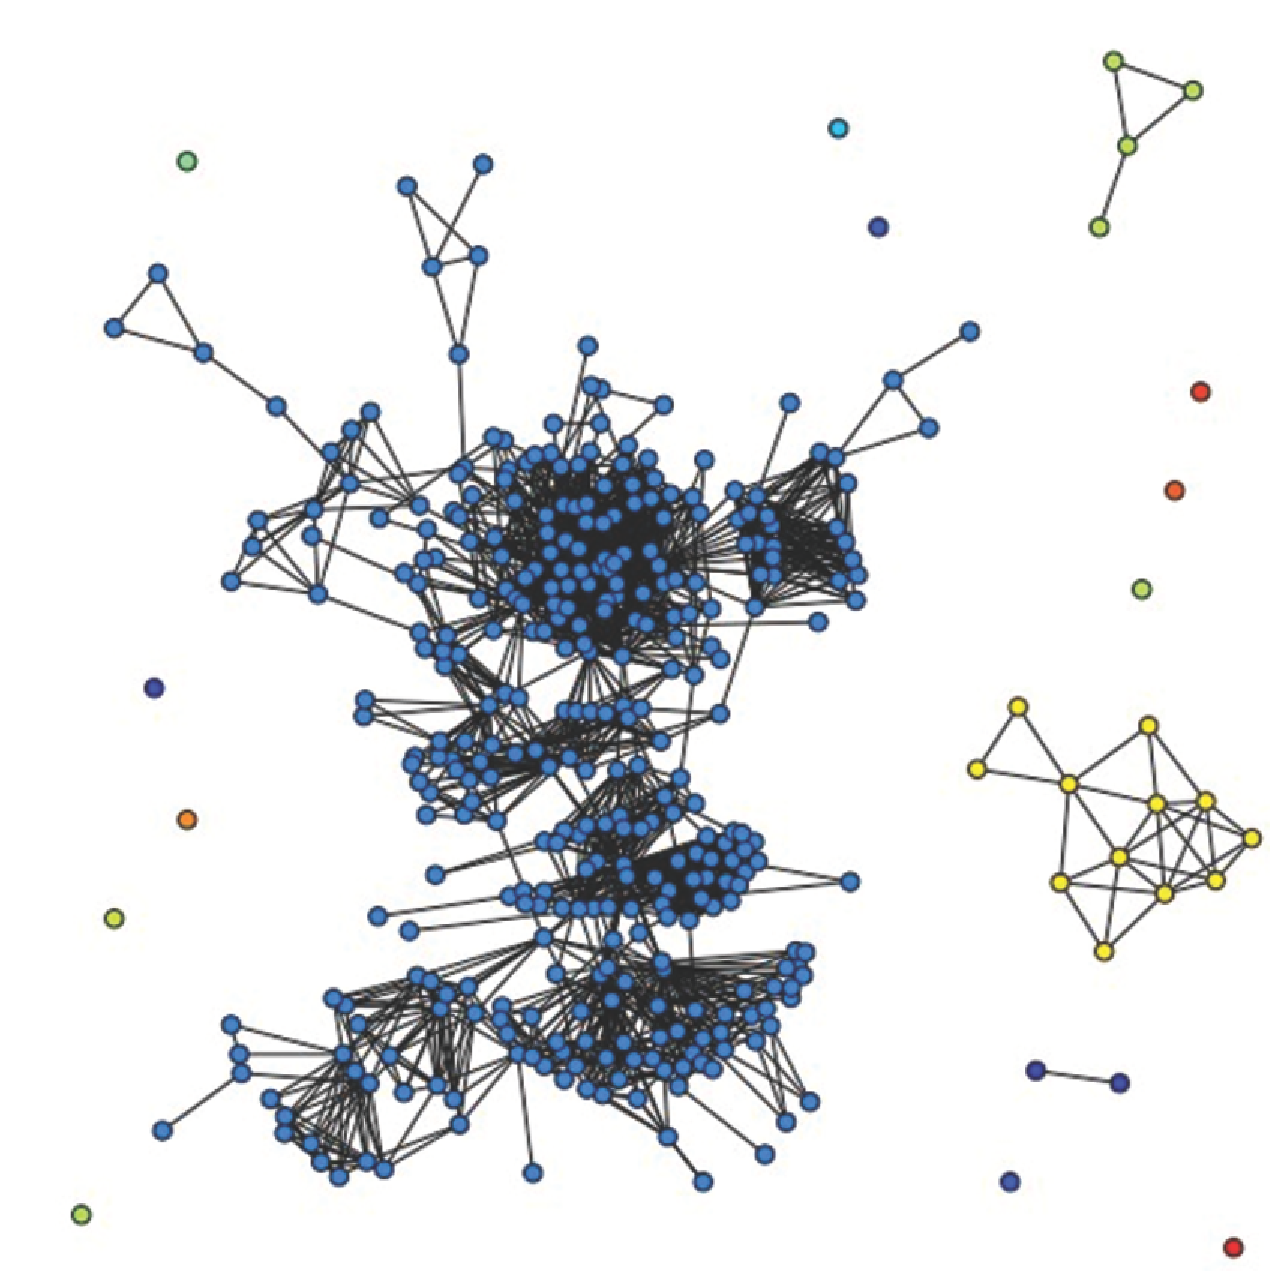
\includegraphics[width=8cm]{Fig1fbnetwork.eps}
\caption{Visualization of a Facebook network}
\label{fig:fbnetwork}
\end{figure}

As shown in figure \ref{fig:fbnetwork}, a Facebook network is represented as a graph where the nodes are the friends of the given users and the connection amongst the
friends are represented as arcs between the nodes of the graph.\\
\\
The mathematical representation of the network graph permits to apply all the techniques of Graph Analysis (a branch of algorithmic mathematics), as described in
\cite{Biggs-1999}.
Mathematically, we can define a Graph as in \ref{eq:graph}:\\

\begin{equation}
G = (V, E)
\label{eq:graph}
\end{equation}

where V is a set of nodes and E a set of edges.
The graphs representing Facebook networks are undirected graphs (if A is friend of B, B is by definition friend of A).
This implies that the elements of E are unordered pairs of elements of V.\\
\\
With this definition we can apply graph theory to study the graph traversal and generation and the complexity of these operations.
Upon this mathematic definition, Social Network Analysis is at this point able to compute measures about social connections.
Different measures can be computed, in the following the measures computed by Rorschach Test Platform will be described.
They can roughly be divided into three sets:
\begin{enumerate}
\item basic indexes;
\item centrality indexes;
\item subgroups indexes.
\end{enumerate}

\label{sec:basicindexes}
\subsection{Basic indexes}
Basic indexes are measures computed on the more direct and visible structural characteristics of the graph.
They can be easily measured from the graph data (nodes and edges) and produce information on the network as a whole
(i.e. these indexes do not refer to any specific node or subset of the network but they refer to the complete network).\\
\\
The Rorschach Test Platform computes four such indexes:

\begin{itemize}

\item \emph{Density}: This index measures the density of the network intended as the number of edges actually present in respect to the total theoretical number of edges.
The density of the network is the ratio of edges present in the network and the total number of possible edges of the network.
A network of N nodes can have a maximum of N * (N-1) edges.

The formula for this index is, then, the one presented in \ref{eq:density}.

\begin{equation}
density(G) = 
\frac{\left | E \right |}
{\left | N \right | * \left ( \left | N \right | + 1 \right )}
\label{eq:density}
\end{equation}

Facebook networks are usually very sparse, so very low values of this index are expected.
Typical values can be around .05 or even less.

\item \emph{Geodesic}: In graph theory, the geodesic distance is the smallest path length between two nodes.
This index, then, measures the average of all the geodetic distances between all connected nodes in the network.\\
\\
This value represents the number of connections each node has to contact in order to reach every other node in the network.\\
\\
Given the definition of geodesic distance between two nodes as in \ref{eq:distance},

\begin{equation}
\begin{split}
distance(v_{1}, v_{2}) = min\left ( d(v_{1}, v_{k}) + d(v_{k}, v_{2}) \right )
\textrm{, } \forall v_{k} \in V \\
\textrm{ where }
d(v_{i}, v_{j})=\left \{
\begin{matrix}
0 \textrm{ if } v_{i} = v_{j} \\
1 \textrm{ if } v_{i}, v_{j} \in E \\
+\infty \textrm{ otherwise}
\end{matrix}
\right.
\end{split}
\label{eq:distance}
\end{equation}

the formula for this index can be expressed as in \ref{eq:geodesic}.

\begin{equation}
geodesic(G) = \frac{\sum_{v_{1}, v_{2}\in V}{distance(v_{1}, v_{2})}}{\left | E \right |}
\label{eq:geodesic}
\end{equation}

This index is lower the more connected the network is. In fact connected networks offer short paths between two randomly choosen nodes.
Typical values for quite strongly connected Facebook networks are around 4.

\item \emph{Fragmentation}: The fragmentation index shows how much the network is fragmented, that is how many node pairs of the network cannot reach other
node in the network.
Thisindex is the ratio of the number of node pairs for which the network does not have a path to connect them.
Nodes not connected may be isolated nodes or nodes belonging to two non connected subgraphs.\\
\\
This index gives an indication about how uniformely the network can be divided.
Very low values indicates networks that shows very few unconnected subparts.
Higher values indicate networks in which different components and subparts can be identified.\\
\\
This index can be computed starting from a matrix of geodesic distances between all the nodes.
This matrix can be computed using the Floyd-Warshall algorithm \cite{Lawler-2001}.

The formula for this index can then be expressed as in \ref{eq:fragmentation}.

\begin{equation}
\begin{split}
fragmentation(G) = count(n_{1}, n_{2}) \textrm{, } \forall n_{1}\in V, n_{2} \in V \\
\textrm{where } distance(n_{1}, n_{2}) = +\infty
\end{split}
\label{eq:fragmentation}
\end{equation}

Usual Facebook values could be quite high, usual social networks have more than one set of nodes (i.e. parents, friends form work, friends from university, ...).
A typical real value for this index could be around .20.

\item \emph{Diameter}: The diameter of a network is the longest geodesic between two nodes randomly choosen inside the network.
This index measure the longest path that can be followed inside the network between its nodes without starting a circle.
The lower this value, the more interconnected the network is.\\
\\
This index is computed from the matrix obtained with Floyd-Warshall algorithm which computes the geodesic distance between each pair of nodes in the graph.\\
\\
The formula for this index can be expressed as in \ref{eq:diameter}.

\begin{equation}
\begin{split}
diameter(G) = max\left ( distance(v_{1}, v_{2}) \right )
\textrm {, } \forall v_{1} \in V, v_{2} \in V \\
\textrm{ where }
distance(v_{1}, v_{2}) \neq  +\infty
\end{split}
\label{eq:diameter}
\end{equation}

Typical values may be around 10. Networks with smaller values are more connected.
\end{itemize}

\label{centralityindexes}
\subsection{Centrality indexes}
Centrality indexes are computed on network nodes and try to express how much each node is ``central" in the nework.
Beying central is a concept of difficult definition.
A node can be central if it has a lot of connections with other nodes, if it is part of most of the shortest paths between other nodes, or for many other reasons.\\
\\
This heterogenity in the definition of the concept of centrality brought to the development of different sociological indexes.
The Rorschach Test Platform computes five different centrality indexes, described in the following.

\begin{itemize}
\item \emph{Degree}: This index is computed evaluating an index of centralization for each node and then computing the mean of this value on all the nodes in the graph.
The centralization for a node is computed by counting the edges each nodes participate to.
Given a node v, its centrality is the ratio of nodes it is connected to, in respect to the total number of nodes of the graph.
The degree centrality value is then computed by calculating the mean of such centrality for each node.\\
\\
The formula for this index can then be expressed as in \ref{eq:degree}.

\begin{equation}
\begin{split}
centralization(v) = \frac{\left | (v, j) \in V \right |}{\left | E \right |}
\textrm{, } \forall j \in V \\
degree(G) = \overline{centralization(v)}
\textrm{, } \forall v \in V
\end{split}
\label{eq:degree}
\end{equation}

This value in Facebook networks is usually very low.
Facebook networks in fact are usually very sparse.
Networks with good levels of connection amongst each node have index values around .03.

\item \emph{Centralization}: This index measures the inequality of degree centrality for all the nodes in the network.
It can be seen as an index for network hierarchy.
The degree centrality for a node is the ratio of nodes it is connected to (in respect to the total number of nodes of the graph).
The degree centrality values are normalized by dividing by the maximum possible degree in a simple graph n-1 where n is the number of nodes in the network.\\
\\
The formula for this index can then be expressed as in \ref{eq:centralization}.

\begin{equation}
\begin{split}
centr(v) = \frac{\left | (v, j) \in V \right |}{\left | E \right |}
\textrm{, } \forall j \in V \\
maxval = max(centralization(v | V) \\
centralization(G) = \overline{maxval - centr(v | V)}
\end{split}
\label{eq:centralization}
\end{equation}

This value on average Facebook networks can vary around .15.
Facebook networks are, in fact, almost equally dense.

\item \emph{Closeness}: This index measures the average closeness for the nodes of the network.
The closeness is measured from the geodesic distance of the node with all other nodes of the network.
Closeness centrality of a node is 1/average distance to all other nodes.
Intuitively, we may say that the closeness measures ``how close" a node is with all other nodes of the network.
Closer nodes are nodes that probably are more tied together and are socially more bound.\\
\\
The formula for this index can then be expressed as in \ref{eq:closeness}.

\begin{equation}
\begin{split}
close(v) = \frac{1}{\overline{distance(v, w | V)}} \\
closeness(G) = \overline{close(v | V)}
\end{split}
\label{eq:closeness}
\end{equation}

In usual Facebook networks, which are very sparse, this values may have typical value of .20.

\item \emph{Eigenvector}: This index measures the average of the centrality for the nodes of the network.
The eigenvector is used to compute this centrality index.
Eigenvector centrality is a measure of the influence of a node in a network \cite{Axler-1997}.
It assigns relative scores to all nodes in the network based on the concept that connections to high-scoring nodes contribute more to the score of the node in question
than equal connections to low-scoring nodes.\\
\\
The formula for this index can then be expressed as in \ref{eq:eigenvector}.

\begin{equation}
\begin{split}
Av = \lambda v \Rightarrow eigen(v) = \lambda \textrm{, with } v \neq 0 \\
\textrm{and A = square matrix } \left | N \right |*\left | N \right |
\textrm{with edge weights} \\
\quad & eigenvector(G) = \overline{eigen(v | V)}
\end{split}
\label{eq:eigenvector}
\end{equation}

Usual values of this index, in Facebook networks, are very low.
Well connected networks have values around .03.

\item \emph{Betweenness}: This index measures the average of the betweenness centrality for the nodes of the network.
The betweenness centrality is the frequency in which a node is on the geodesic between all the nodes of the network.
Betweenness centrality of a node is the sum of the fraction of all-pairs shortest paths that pass through it.\\
\\
The formula for this index can then be expressed as in \ref{eq:betweenness}.

\begin{equation}
\begin{split}
between(v) = \sum_{v_{1},v_{2} \in V} \frac{\sigma(v_{1}, v_{2}|V)}{\sigma(v_{1}, v_{2})} \\
betweenness(G) = \overline{between(v | V)}
\end{split}
\label{eq:betweenness}
\end{equation}

Facebook networks which have this value high (around .10 or even more) are networks in which few nodes are the key elements that keeps all the network connected.
\end{itemize}

\label{sec:subgroupsindexes}
\subsection{Subgroups indexes}
Subgroups indexes evaluate the structure of the network identifying its subparts, cliques and components.
These index family is intended to measure how much the network is completely integrated or, on the contrary, divided into smaller networks of nodes strongly connected
with each other.

\begin{itemize}
\item \emph{Cliques}: This index measures the number of cliques of the network.
A clique is a subset of the graph with at least three nodes and having every node connected with every other node in the subset.
The higher the number of cliques, the more connected the network is.
This index value is heavily influenced by the total number of nodes of the network.
In fact, bigger networks have more probability to create cliques.\\
\\
The formula for this index can then be expressed as in \ref{eq:cliques}.

\begin{equation}
\begin{split}
cliques(G) = \left | (v_{1}, v_{2}, ..., v_{n} \right | \\
\textrm{ with } v_{1} \in V, v_{2} \in V, ..., v_{n} \in V \\
\textrm{ and } (v_{i}, v_{j}) \in E \textrm{, } \forall i, j \textrm{ in } 1...n
\end{split}
\label{eq:cliques}
\end{equation}

A well connected Facebook network has usually a high number of cliques.
A typical Facebook network of 400 nodes, may have this index with a value of 1000.

\item \emph{Comembership}: This index measures for each node pair the number of cliques in which they appear together.
The sum of the comembership for each node pair is then divided by the total number of possible node pairs: N * (N-1).\\
\\
The formula for this index can then be expressed as in \ref{eq:comembership}.

\begin{equation}
\begin{split}
cliqueset(G) = (v_{1}, v_{2}, ..., v_{n} \\
\textrm{ with } v_{1} \in V, v_{2} \in V, ..., v_{n} \in V \\
\textrm{ and } (v_{i}, v_{j}) \in E \textrm{, } \forall i, j \textrm{ in } 1...n \\
comembership(G) = \left | \left ( S | cliqueset(G) \right ) \right | \\
\textrm{where } v_{1} \in S \textrm{ and } v_{2} \in S
\end{split}
\label{eq:comembership}
\end{equation}

Facebook networks which are strongly connected usually present only a small set of dense subgraphs.
These networks have this value higher than other networks (more loosely connected or with more numerous sub-groups).
However, the value of this index is always quite low; a typical value for this index could be .35.

\item \emph{Components}: This index measures the number of components of the network.
A component is a subset of the graph nodes which are connected between themselves and not connected to other nodes in the graph.
This index represents the number of sub-groups present in your Facebook network.\\
\\
The formula for this index can then be expressed as in \ref{eq:components}.

\begin{equation}
\begin{split}
components(G) = \left | (v_{1}, v_{2}, ..., v_{n}) \right |\\
\textrm{ with } v_{1} \in V, v_{2} \in V, ..., v_{n} \in V \\
\textrm{ and } distance(v_{i}, v_{j}) \neq +\infty \textrm{, }
\forall i, j \textrm{ in } 1...n
\end{split}
\label{eq:compoents}
\end{equation}

The value for this index of a Facebook network is small in respect to the number of nodes.
For instance a typical value for a network with 400 nodes could be 20.
\end{itemize}

\label{sec:overallfeatures}
\section{Overall features of the developed platform}
The Rorschach Test Platform, as seen, aims to integrate sociological index calulations performed with SNA techniques, with the results of psychological tests in order to
enrich with useful variables the experimental design.
This platform is well suited for performing social psychology testing but could also be used in other researches.\\
\\
To date the application has not been used in real testing activities, but the plan is that of finding suitable researchess that could benefit from the platform.
The application, however, has been visited by some user who computed his own sociological indexes and network statistics.
As it seems, even without relevant publicity, the social characteristics and the activities on Facebook's timelines are good elements to attract curious visitors to
the platform.\\
\\
In this section all the major features of the Rorschach Test Platform will be presented and described.

\subsection{Test Definition}
The Rorschach Test Platform is born with the aim to ease and facilitate test submission and execution.
The platform has functionalities to permit test definition and, after that, to support test execution.\\
\\
To perform real tests the Rorschach Test Platform leverages the OpenSesame project who has been designed and developed with the aim to ease test construction.
A specific plug-in has been developed to integrate the OpenSesame platform with the Rorschach Test Platform and to permit test administration and SNA index computation.\\
\\
The users defined as administrators of the platform are able to create new tests that can than be associated to steps defined inside OpenSesame.
Such definition on Rorschach Test Platform is requested to guarantee that the experimenter who tries to gatehr such information is really registered as an administrator
of the Rorschach Test Platform and is not trying to access un-authorized information about subjects' social networks.\\
\\
Tests on the Rorschach Test Platform are created by specifying:
\begin{itemize}
\item a unique test name;
\item a test description;
\item a test start date, which is the beginning date for the dispensation of the test;
\item a test end date, which is the end date for the dispensation of the test;
\item an OpenSesame test file, which can optionally be uploaded to ease test distribution.
\end{itemize}

Each test can be marked, in the Rorschach Test Platform, as active or inactive.
Every user accessing the platform will see all valid tests.
A test is considered to be valid if it is marked as active and if the current date is within the start and the end date for the test.\\
\\
Once the test has bee created inside Rorschach Test Platform, the specific plugin inside OpenSesame must be properly configured.
The plugin can be downloaded directly from the Rorschach Test Platform Facebook application.\\
\\

\begin{figure}[h]
\centering
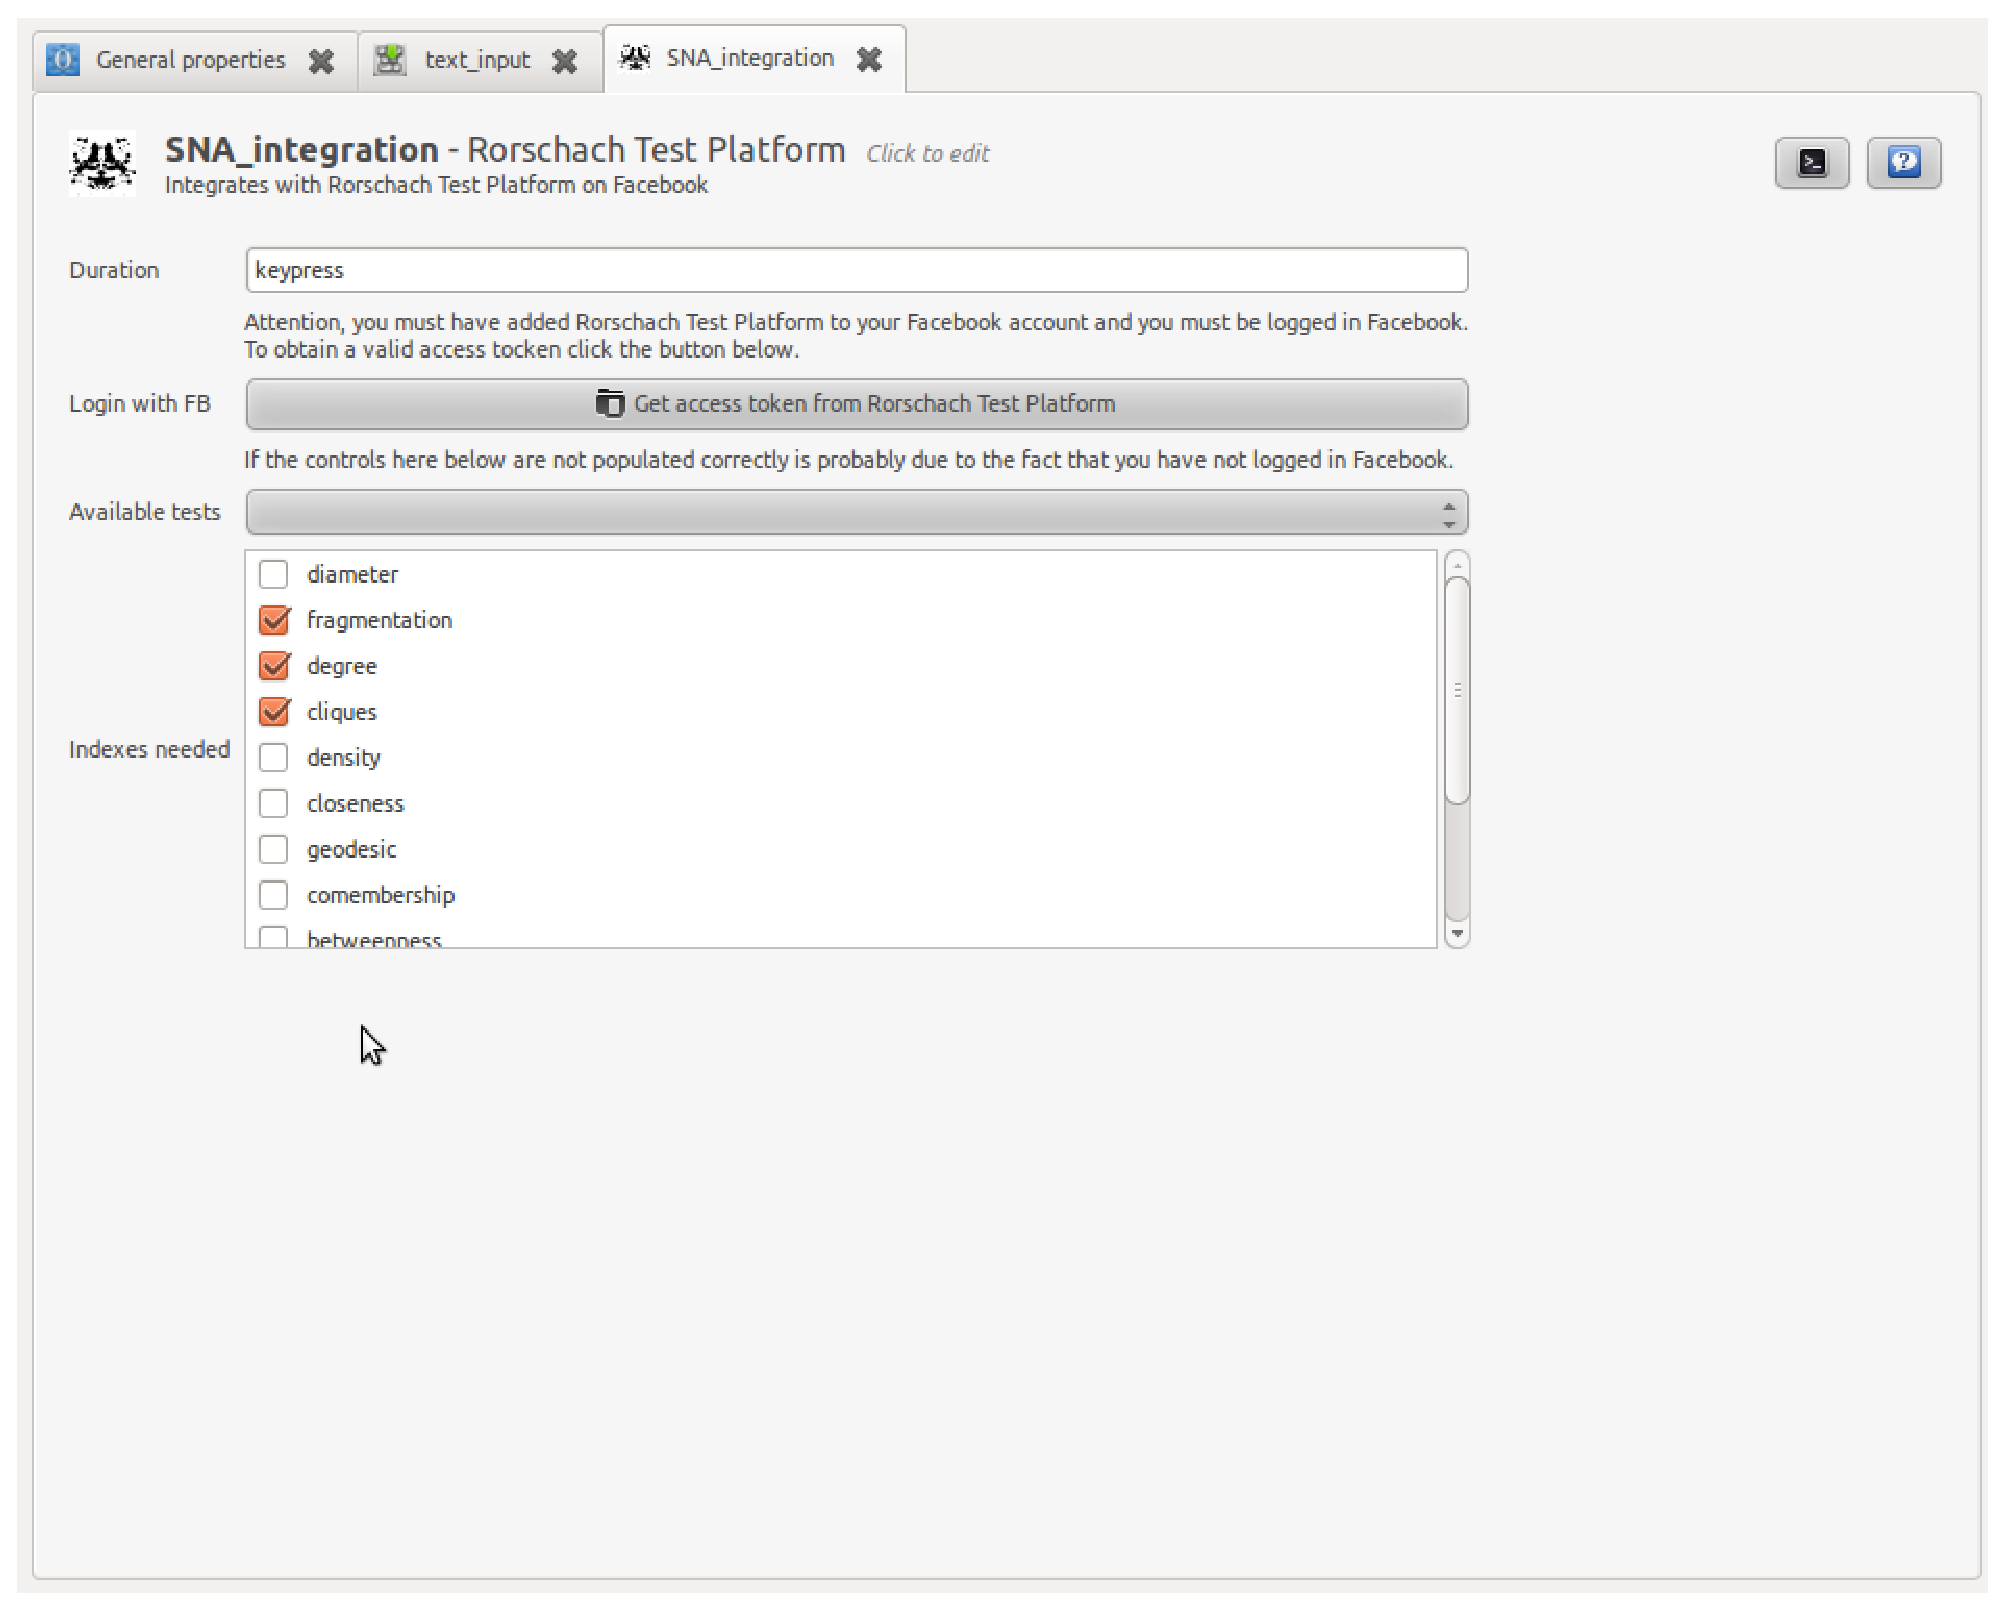
\includegraphics[width=12cm]{Fig2testconfig.eps}
\caption{Configuration of the Rorschach Test Platform plugin inside OpenSesame}
\label{fig:testconfig}
\end{figure}

Once installed, the plugin must be added as a step in the test.
The plugin is available in the ``Response collection" set of items inside OpenSesame.
The configuration, as shown in figure \ref{fig:testconfig}, needs the following steps:

\begin{itemize}
\item Duration: the duration permits to configure how long the information about the downloaded indexes are presented to the subject during the test execution.
Downloaded indexes, added as variables to the tests, are intended to be shown to the subject.
This parameter permits to configure how long the recap screen will be visible to the subjects.
The possible values for this field are the duration in milliseconds or `keypress' or `mouseclick' to indicate that the data screen will remain present to the user as
long as he presses a key on the keyboard or presses a mouse button.
The experimenter can also specify `hidden' on this parameter to mean that the recap screen is not shown to the subject.
\item Login with FB: in order to integrate with the Rorschach Test Platform, this plugin has to authenticate the user as a proper administrator of the platform.
This login operation is performed by clicking this button and following the normal login operations inside the browser window that will open consequentely.
The user will be asked to login to Facebook and to access the Rorschach Test Platform application to verify he is actually an administrator on such platform.
\item Available tests: after having logged in with Facebook, this dropdown menu shows all available tests, defined in the platform.
The user is asked to associate the OpenSesame test with a valid test on the Rorschach Test Platform.
\item Indexes needed: this listbox shows all the sociological indexes computed by the Rorschach Test Platform and permits to check the ones needed in the test being configured.
\end{itemize}

After these configurations, the researcher will continue to set up his/her test inside OpenSesame and will submit it to the intended research population.
The test can even be uploaded to the Rorschach Test Platform in the test definition so that the users can easily download and run it on theri OpenSesame platform.

\label{sec:testexecution}
\subsection{Test Execution}
The test execution is performed in the OpenSesame platform as for a standard test.
The subject running the test, passes through two phases in the execution:

\begin{enumerate}
\item prepare phase: this phase is inteded to prepare all test steps so that they can be executed by the subject;
\item run phase: this phase is the actual run phase, which can be measured in time and gathers all test data.
\end{enumerate}

The Rorschach Test Platform plugin, for the subject running the test, needs to perform different operations in the two phases.
In the prepare phase the plugin has to authenticate the user with Facebook and the Rorschach Test Platform application.
This is performed, as during plugin configuration, directly inside a browser window opened by the plugin.\\

\begin{figure}[h]
\centering
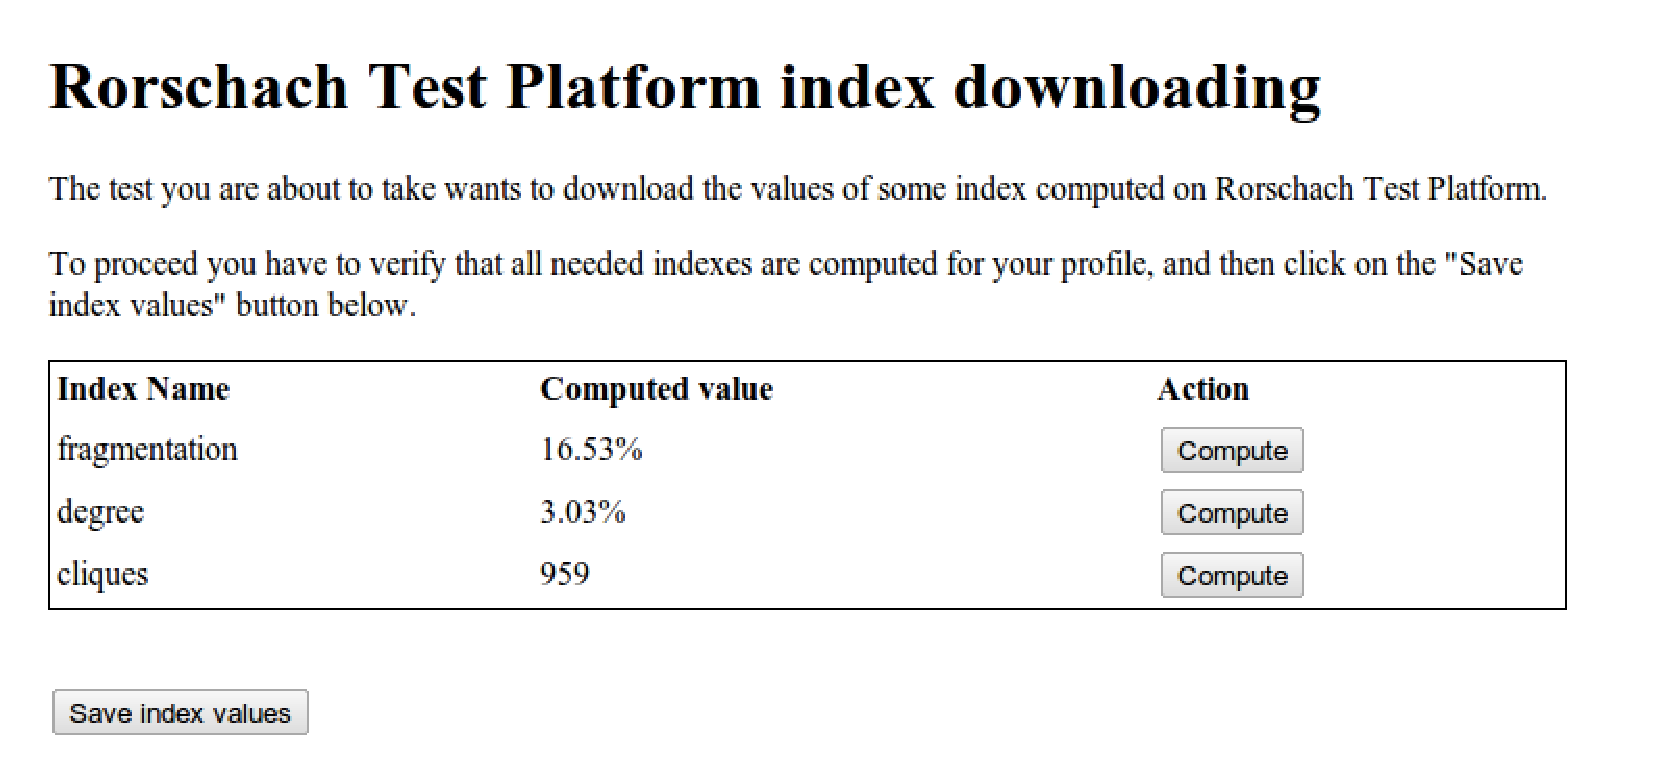
\includegraphics[width=12cm]{Fig3indexeval.eps}
\caption{Test preparation phase in Rorschach Test Platform plugin}
\label{fig:indexeval}
\end{figure}

As shown in figure \ref{fig:indexeval}, in this window the user is requested to login to the Rorschach Test Platform application and verify that all the indexes requested
by the test have been computed.
For computed indexes, the value is showed.
The subject from this page is able to run the computation for all missing indexes before the test execution phase is actually started.\\

\begin{figure}[h]
\centering
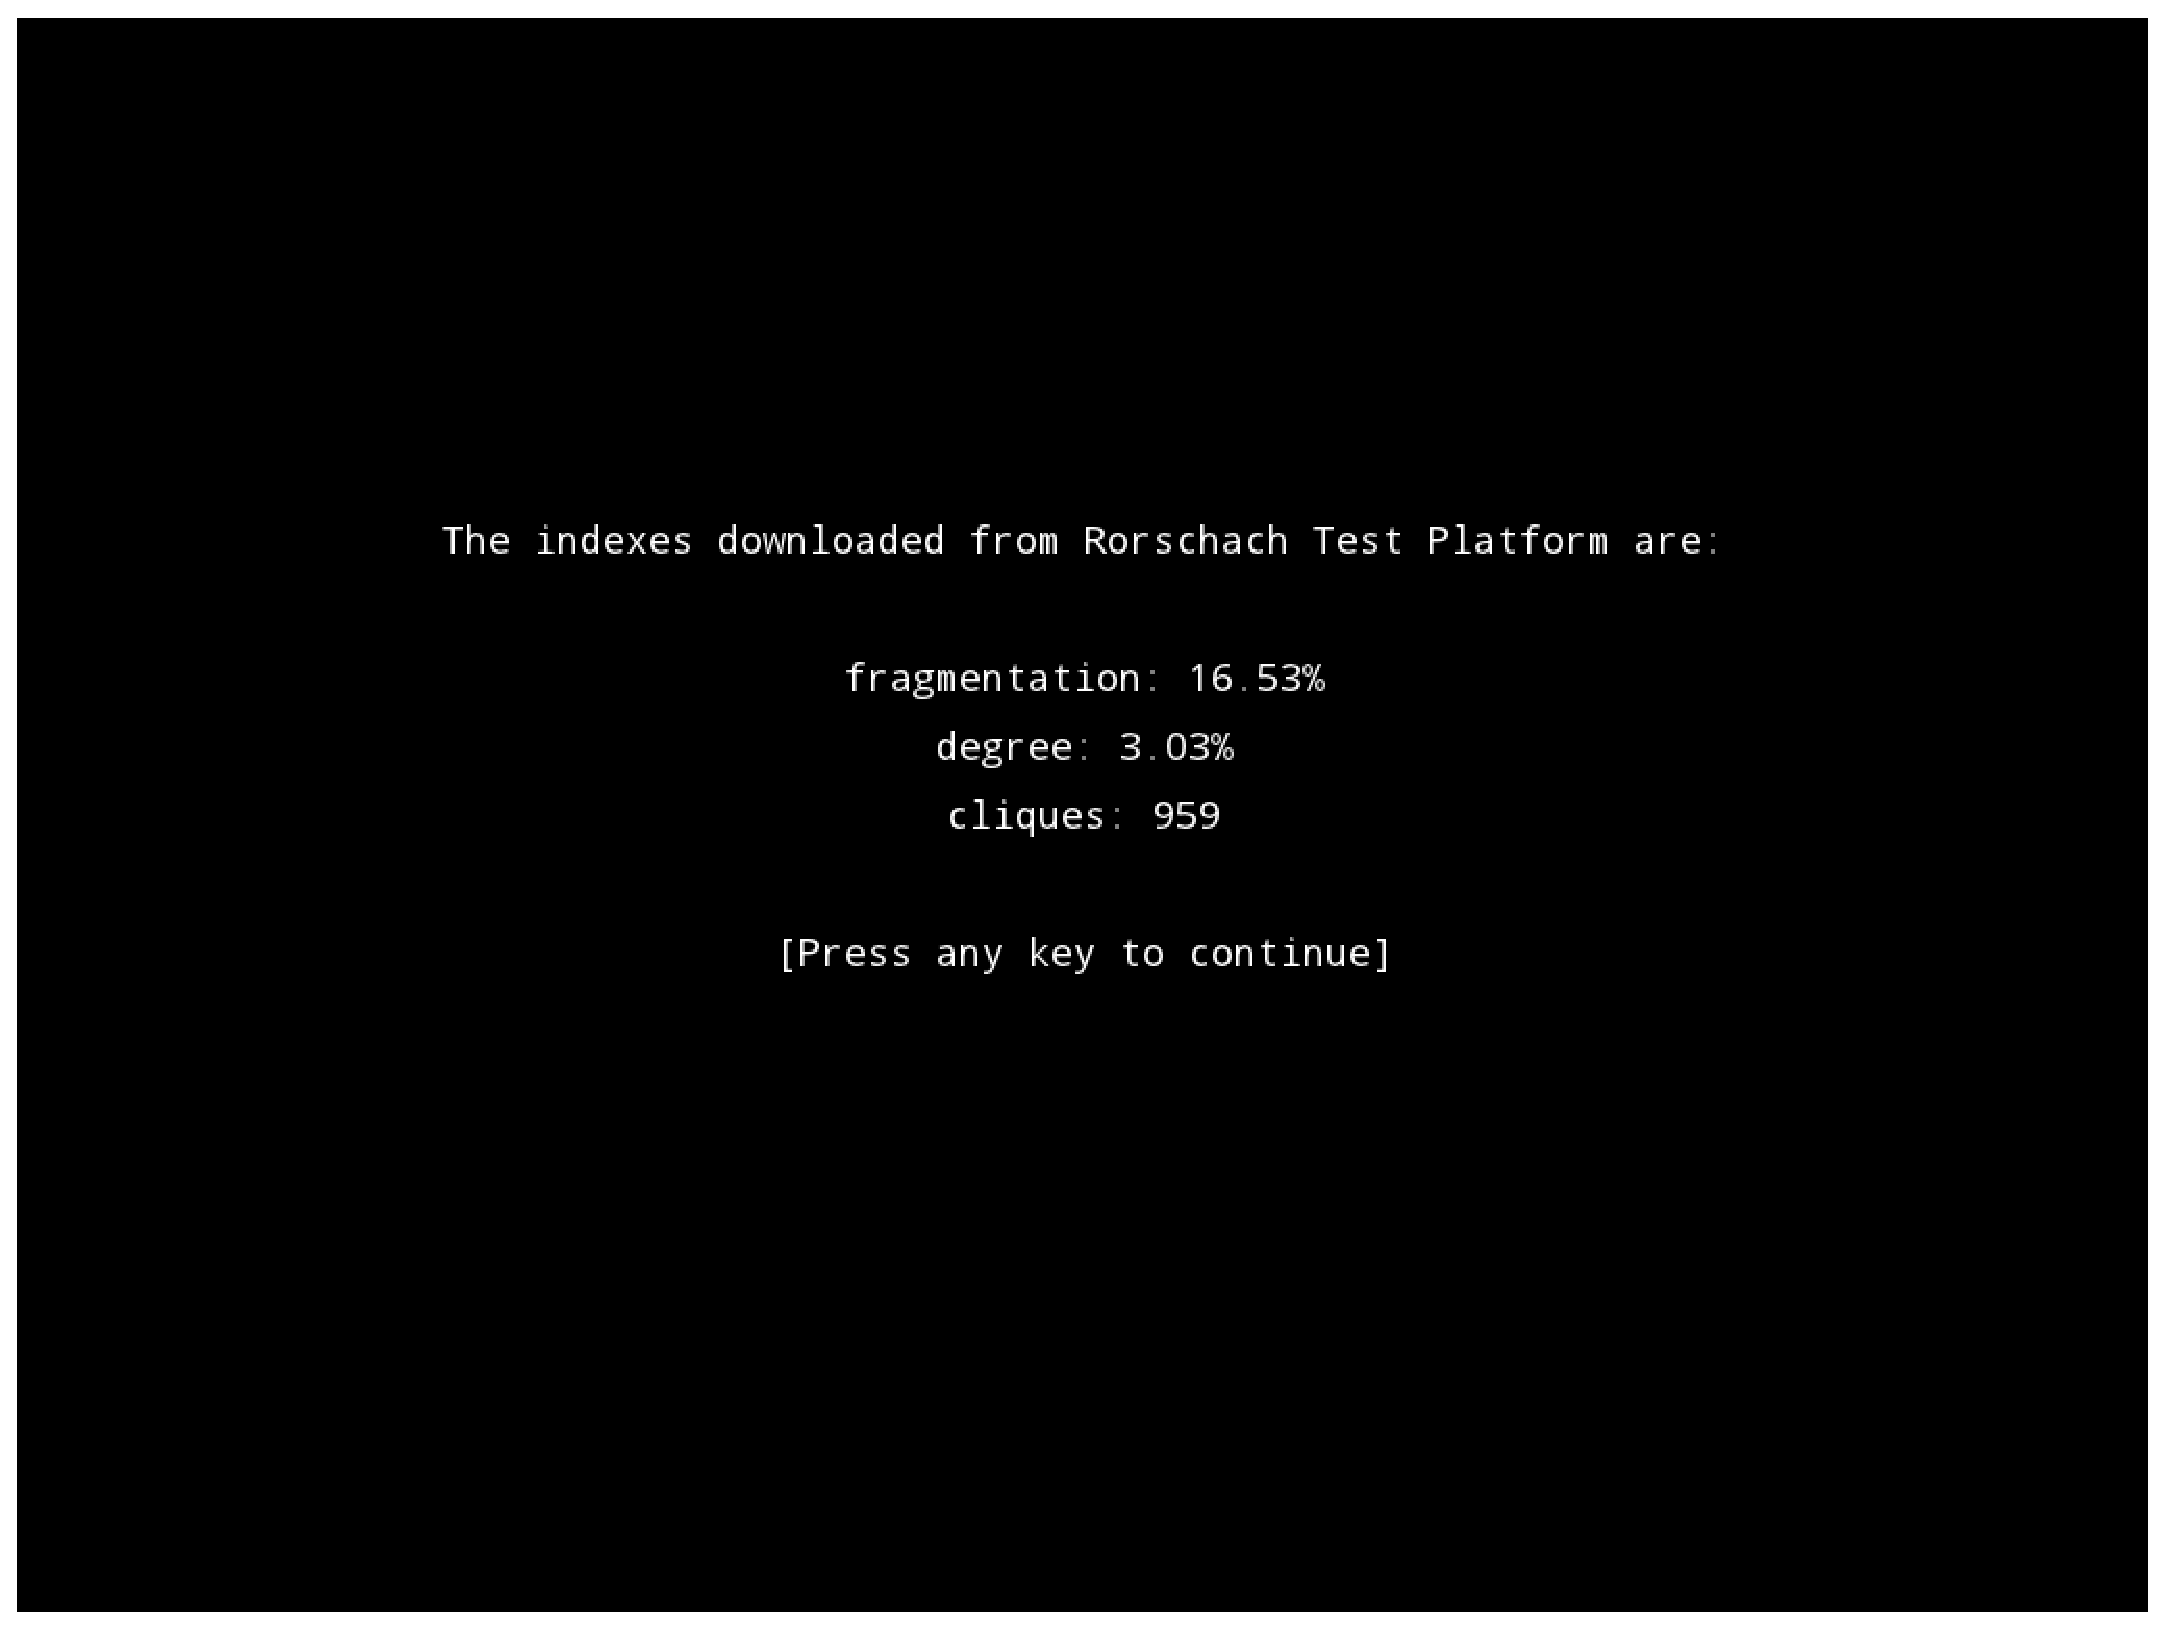
\includegraphics[width=12cm]{Fig4testrun.eps}
\caption{Test run phase in Rorschach Test Platform plugin}
\label{fig:testrun}
\end{figure}

During the test execution, as shown in figure \ref{fig:testrun}, the subject is only presented a screen showing the computed values for the indexes requested by the test
and is asked to continue during the further steps in the text execution.

\label{sec:sociologicalprofile}
\subsection{Sociological profile and index computation}
From the Rorschach Test Platform, each user can check and see its personal sociological profile.
The profile and indexes are visible and can be computed even not during a specific test execution phase.
The profile is composed by the 12 different sociological indexes explained in section \ref{sec:centralityindexes}.
A user accessing his profile will be presented a page similar to the one in figure \ref{fig:profile}.

\begin{figure}[h]
\centering
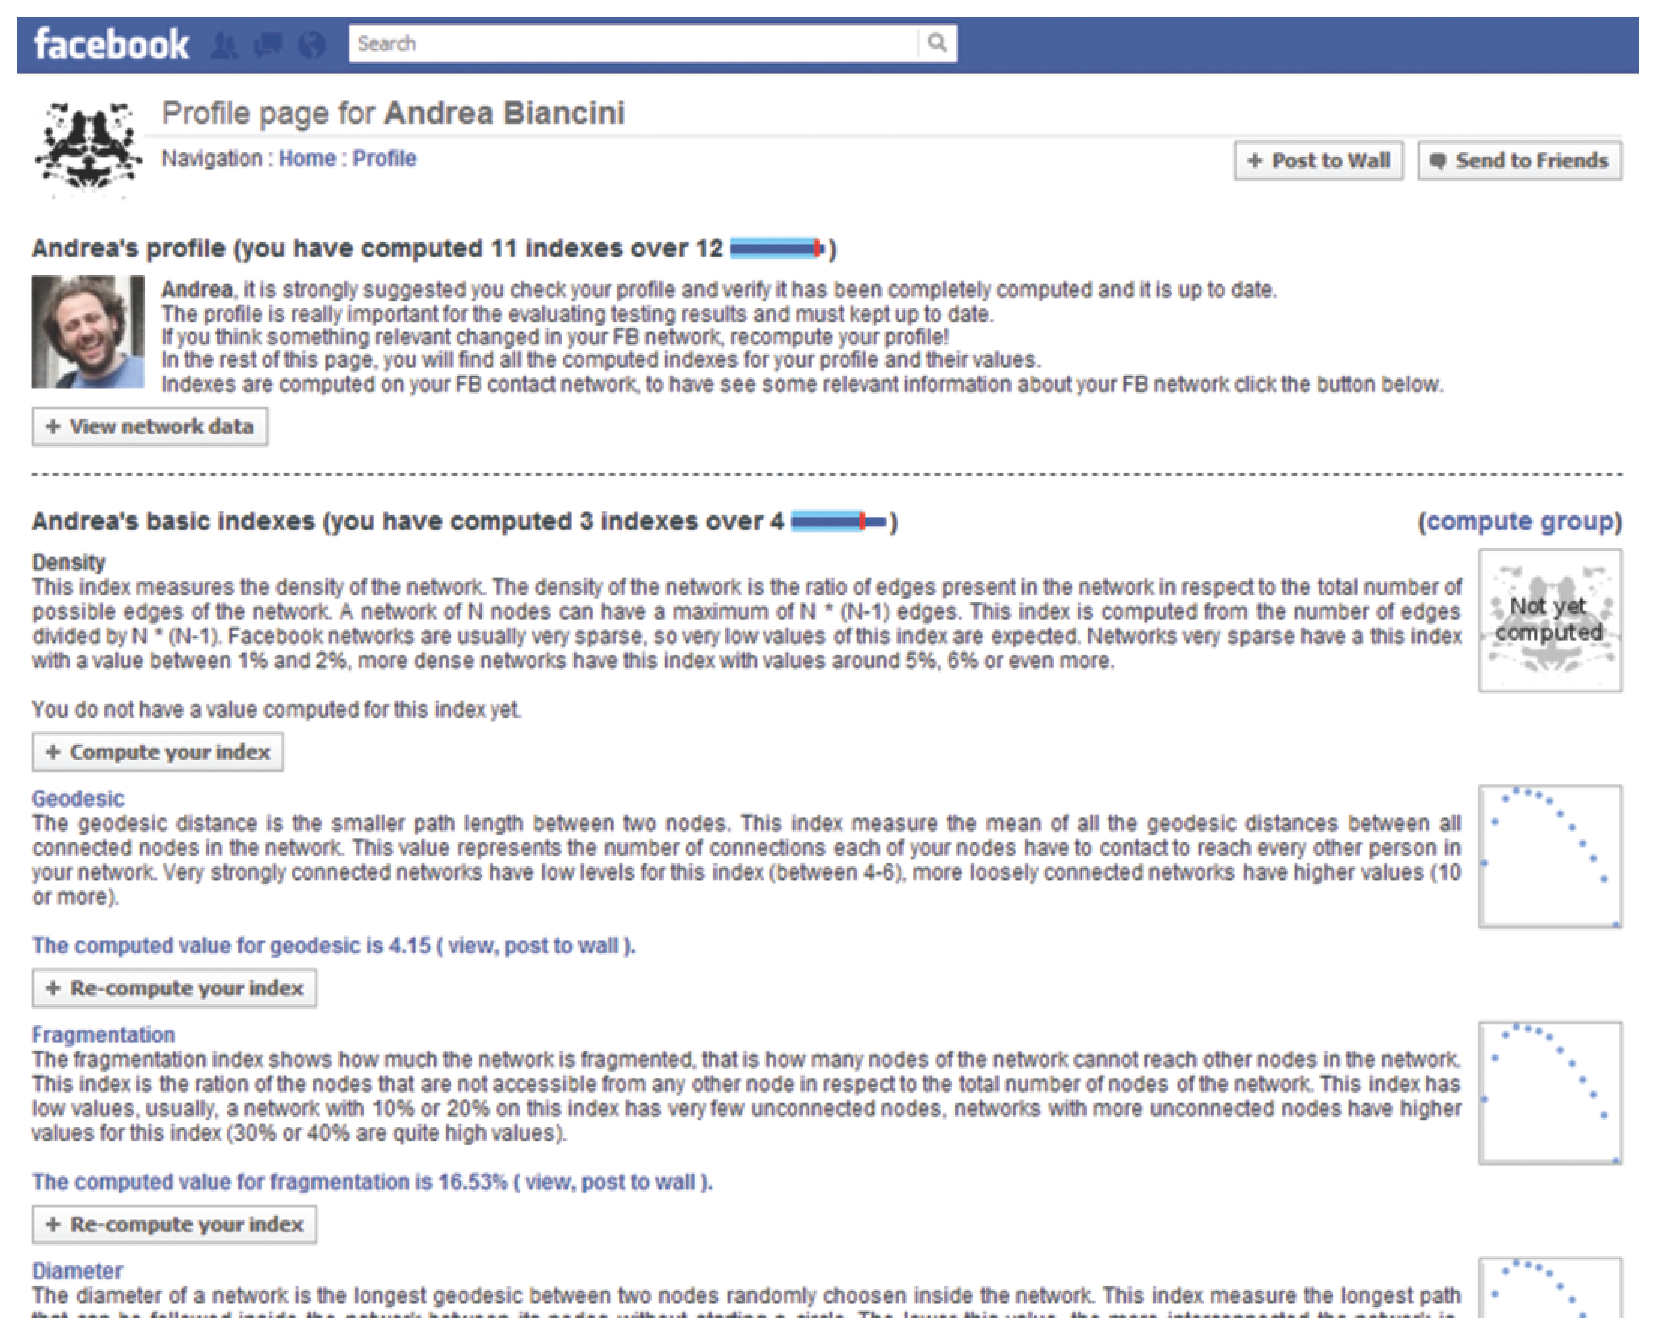
\includegraphics[width=12cm]{Fig5profile.eps}
\caption{An example of a user profile page}
\label{fig:profile}
\end{figure}

From this page all computed indexes shows their value and a distribution graph, over 100 buckets, of nodes or edges (depending on the meaning of the index).
Indexes which are not yet computed can be calculated starting from user's network data downloaded from Facebook.\\
\\
The index computation is executed online.
For users with a number of Facebook contacts not too big (less than 500), the computation is executed on the fly without big delays in user experience.
For users with bigger networks, instead, the computation of sociological index could take longer.
For this reason, in order not to leave the user waiting for an online answer, computations in this case are sent in background and the user is suggested to check
in few minutes to view the computed results.\\
\\
This page also permits to compute all the index in one group (instead of computing them one by one).
The link ``compute group" performs exactly this operation.
In this case the multiple parallel computations, are sent in the background and, as for users with large networks, the platform suggests to come back in few minutes
to view the computed values.
In order to give the users a visual feedback on the status of computation of their profile, coloured progress bars are presented.
They indicate the ratio of indexes computed on the whole profile and for each index group.\\
\\
The platform does not provide a functionality to compute all indexes in parallel.
This functionality has not been implemented for an explicit choice.
It has been considered preferable not to give this possibility, in order to grow user consciousness on his/her sociological index values.
Most of the social interactions implemented by the Rorschach Test Platform, turn around these sociological indexes.
So a higher attention and an active involvement of the user during the computation is preferable to permit a good social diffusion of the platform.

\label{sec:graphvisualization}
\subsection{Graph visualization and friend comparison}
From the index page, the user has the opportunity to see a specific page for each index.
This detailed page shows more information about the index.
It shows the computed overall value and then the information about nodes or edges buckets.
The index computed can refer to nodes or edges of the graph associated to the social network.
In either case the nodes/edges are grouped in 100 buckets depending on the respective value computed during the index evaluation.\\
\\
Apart from a table view of the values for the 100 buckets, this page shows also two graphs of these data.
The two graphs are:
\begin{itemize}
\item a scatter graph showing the distribution of nodes or edges over the buckets (an example in figure \ref{fig:scatter});
\item a bar graph showing the number of nodes or edges for each bucket and a line showing the normal distribution of values over the bucket
(an example in figure \ref{fig:gaussian}).
\end{itemize}

\begin{figure}[h]
\centering
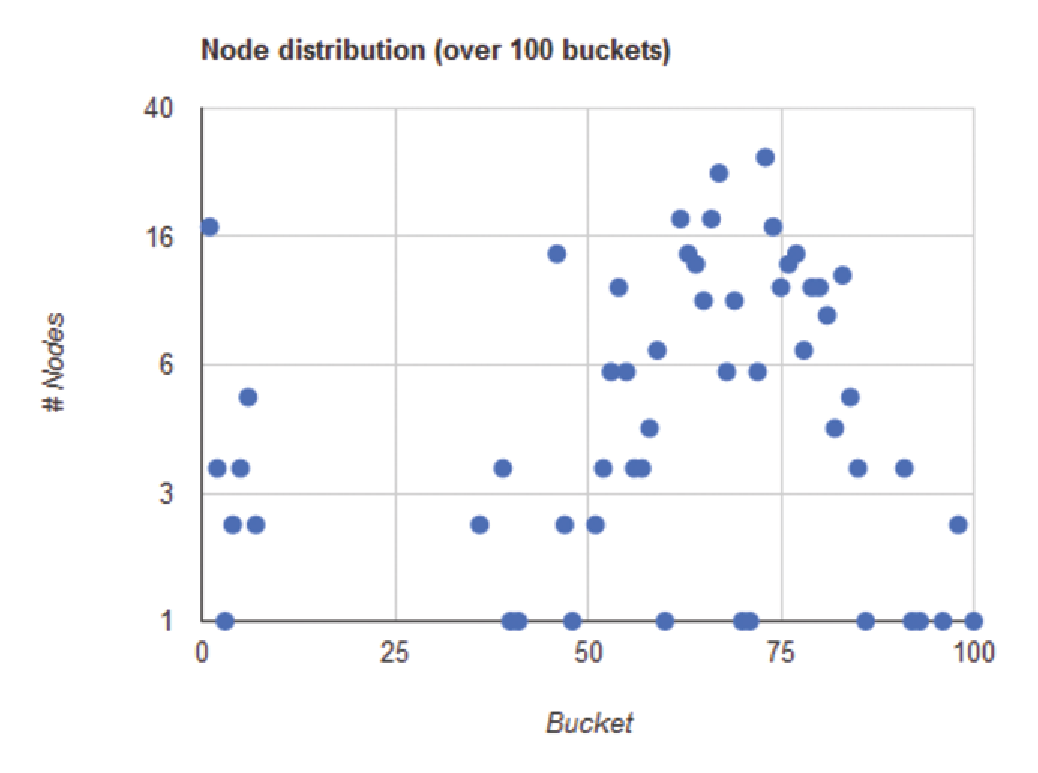
\includegraphics[width=8cm]{Fig6scatter.eps}
\caption{Example of a scatter node bucket graph for an index}
\label{fig:scatter}
\end{figure}

\begin{figure}[h]
\centering
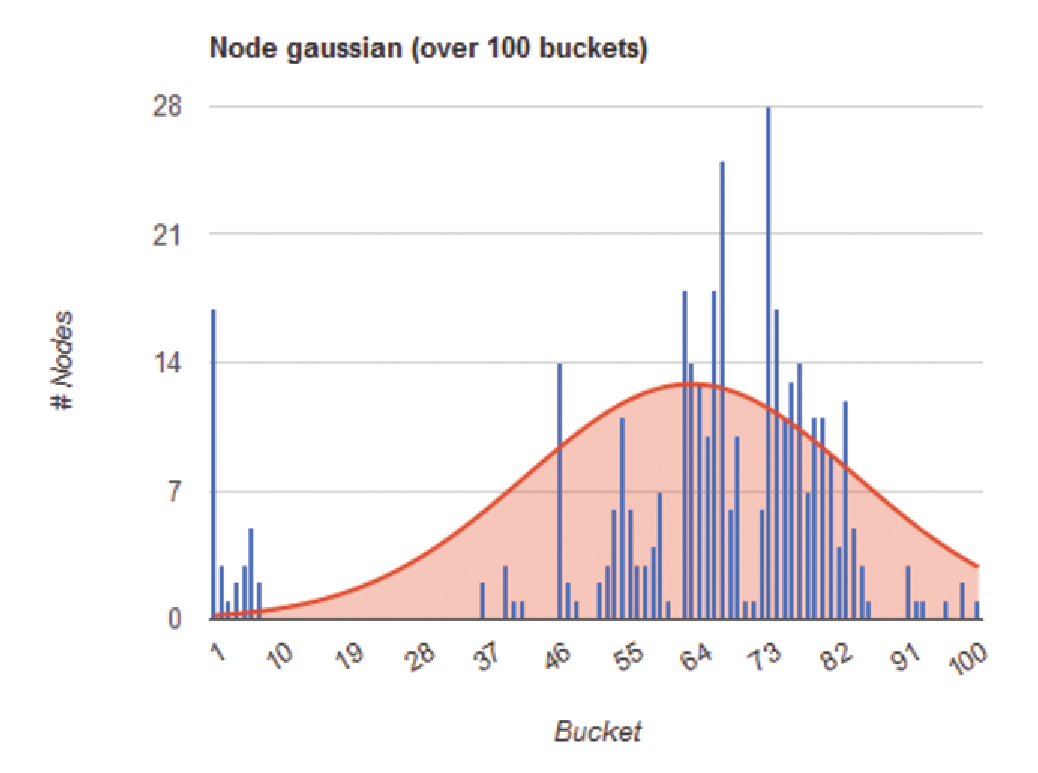
\includegraphics[width=8cm]{Fig7gaussian.eps}
\caption{Example of a gaussian node bucket graph for an index}
\label{fig:gaussian}
\end{figure}

These information should help to tease the curiosity of the users and then nourish the desire to share this data with friends and on Facebook timelines.
In this sense, this index page pemits also to perform comparisons of our index value with the one of some friend which is also using the Rorschach Test Platform.
When the user performs a comparison, the index value computed on the friend's network is shown side by side with his/her own.
Moreover the graphs show a comparison of the bucket distribution of the values for two users.
In figure \ref{fig:comparison}, an example of the gaussian graph is provided which shows the comparison with a friend's values.

\begin{figure}[h]
\centering
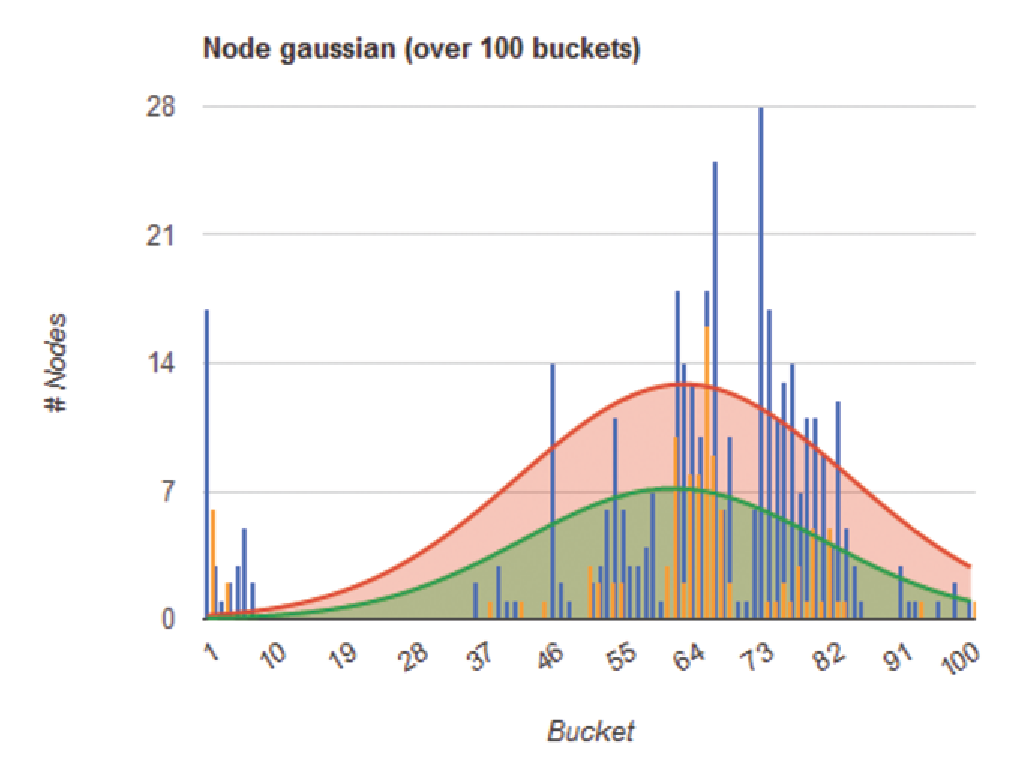
\includegraphics[width=8cm]{Fig8comparison.eps}
\caption{Example of a gaussian comparison graph}
\label{fig:comparison}
\end{figure}

\label{sec:netstatistics}
\subsection{Network statistics visualization}
The Rorschach Test Platform, from the profile page, permits also to show some data about the network shape and characteristics.
By asking to see his/her own network data, the user is presented with some basic information about his Facebook contacts network.\\
\\
The basic information presented consist of two values.
At first the user is shown the number of nodes (i.e. friends) present in the network.
In addition, the user is also shown the number of edges (i.e. connections amongst friends) in the network.
These information are very basic, but permit to have a feeling of the size of the Facebook network.\\
\\
Beside these information, a sort of friend league is presented.
This table (which shows more or less 20 friends) is intended to provide a sort of elite group of a user's Facebook network.
This elite group is not intended, and could not be able to, represent a realistic scale of the user's social relationships.
It instead shows the top nodes on your network based on the values of three indexes.\\
\\
The three indexes (already described in 3.1) used to evaluate this elite network are:
\begin{itemize}
\item degree: which shows the number of connections the node has in the network;
\item closeness: which computes “how close” a node is with all other nodes of the network;
\item betweenness: which computes the frequency in which a node is on the geodesic between all the nodes of the network.
\end{itemize}

From this three index values, for each node a total score is computed giving the higher prevalence to the degree index, then closeness and at last betweenness.
All the nodes are then ordered on this computed score and the top ones are presented to the users as the elite group.

\label{sec:fbintegration}
\subsection{Facebook integration}
The Rorschach Test Platform has some feature aimed to promote the platform itself.
These ``promotional" features are intended to permit, via the growing of the usage of the platform, the highest possible diffusion of the tests dispensed on it.
The very nature of the platform, built as a Facebook application, makes straightforward to use Facebook social mechanisms to try achieve a higher distribution.\\
\\
The platform, then, strives to integrate at best with the Facebook platform and to attract a large number of users in using it.
The integrations with Facebook are at various levels and are aimed to obtain a true sociological design for the platform itself.
The areas of social integration of the platform within Facebook are the following:

\begin{itemize}
\item On the homepage of the application, the user is recognized, greeted by its name and his Facebook profile picture is shown.
\item Again on the homepage, a list of friends is shown which already use the application.
\item As seen in section \ref{sec:overallfeatures}, the user is given the opportunity to compare his/her index and network values with the ones of another friend.
\item Form different points of the application the user can decide to post some information on his/her timeline.
The information that can be posted are about index values or network elite groups.
\item The application integrates with the new Facebook APIs called Open Graph.
These APIs permit to create entities and actions over them that are then shown on the user timeline.
The Rorschach Test Platform defines entities for by the sociological indexes and the Facebook network of the users.
\end{itemize}

\label{sec:conclusion}
\section{Conclusion and future developments}
The platform described in this article, has been developed to sustain social testing researches.
The work performed so far started from the assumption that leveraging the Facebook platform it would be possible to obtain two important benefits:

\begin{enumerate}
\item on one side, it is possible to diffuse tests very easily, rapidly and with very small costs;
\item on the other side, Facebook contains a lot of information about the social behavior of its users wich can be used to enrich psychological researches.
\end{enumerate}

The platform developed integrates with OpenSesame which is an open source project with the aim to define and execute social science tests.
The Rorschach Test Platfrom showed the possibility to use Facebook in a smart way, to ease test diffusion and to integrate test data with relevant sociological
information on users' Facebook networks.\\
\\
In future works some deeper integration with Facebook can be studied and achieved.
Currently, the application computes indexes only on the static configuration of network connections.
Facebook, however, contains a lot of other information about the user behaviors.

This more dynamic data, at the moment, is not collected and used by Rorschach Test Platform.
In the future, it should be interesting to develop the features needed to calculate indexes that model the user behavior.
The information stored by Facebook is, for example, posts on friend's timelines, photoes upload and tagging, likes on pages and comments of other users.\\
\\
Finally, the platform could be used to put together sociological information of a consistent number of users.
This could help in building a sociological normative database to be used to better incanalate future developments and evolutions of the platform and of researches in this area.

\section*{Acknowledgements}
The author would like to sincerely thank Prof. Marco Paganoni for his support and continuous help in working on such projects and activities.

\appendix
\label{sec:techdesign}
\section{Technical design of the platform}
In this section the relevant technical aspects of the platform are described.
The platform itself is build as a Facebook application (view \cite{Facebook-2011}) and is hosted on Google App Engine cloud platform (\cite{GAE-2011}).
The platform, called Rorschach Test Platform in honor of the swiss psychiatrist and psychoanalyst Hermann Rorschach and its inkblots projective test,
is pubblicly accessible on Facebook (\cite{Rorschach-2011}).

\label{sec:GAE}
\subsection{Google App Engine}
Google App Engine (GAE) is a Platform as a Service cloud service offered by Google which enables to build and host web applications on the same systems that power
Google applications.
For the realization of the Rorschach Test Platform, GAE has bee used because of many benefits it could offer directly:

\begin{enumerate}
\item the GAE platform is very simple and offers an easy to use web-based dashboard that makes it simple the management of the developed applications;
\item GAE enables an application to scale automatically without the need to worry about managing machines and other infrastructure elements;
\item the GAE platform has a very modular cost scheme, all the development and small testing can be performed with no cost.
Further utilization of the application for real user experience can be done with controlled and limited costs.
\end{enumerate}

The GAE platform permit to realize very quickly a full featured web-site that works as a Facebook application.
Moreover, GAE offers a pesistent storage that permits to memorize user data (in terms of test answers and sociological index information).\\
\\
Google App Engine, as a cloud platform, is also able to perform automatic scaling and load balancing.
This is an important feature for this application which could need extra capacity to permit a widespread test analysis upon large number of subjects.
This high scalability is made possible by leveraging on a high number of parallel servers which could respond to different user requests.
This horizontal scalability is very effective on internet applications but is not designed to support heavy computations.
The computation of sociological indexes on big Facebook networks needs more time and this could represent a problem for users which could experience delays and
slowdowns in their experience.
To circumvent this problem GAE offers the possibility to use task queues that perform work outside of the scope of a web request.\\
\\
Finally, GAE offers a feature that permits to execute scheduled tasks for triggering events at specified times and regular intervals.
This feature has been used by the Rorschach Test Platform to perform cleaning and tidying operation on the application data offline.\\
\\
App Engine offers different application environments to be used.
The more relevant of those are Java 6 and Python 2.7 runtimes.
For this platform the Python environment has been used.
App Engine includes rich APIs and tools for Python web application development, such as Django.
The Python environment includes the Python standard library and some third-party libraries (such as NumPy heavily used in the platform to perform calculations
on matrix and graphs).

\label{sec:fbintegration}
\subsection{Facebook integration}
One of the most relevant advantages of Rorschach Test Platform is its integration with Facebook to retrieve relevant user information to perform social index computation.
The entire Rorschach platform is basically a Facebook application and, as such, is able to query and obtain information about its users.\\
\\
The overall Facebook integration mechanism works around the concept of Facebook application.
An application is defined by a couple of keys (an access key and a secret key) that are used to authenticate users and query the platform to retrieve data.
When a user access a Facebook application for the first time, an authorization dialog appears asking to grant the application the rights to access information and user
data on Facebook platform.\\
\\
Facebook as an application platform, provides different mechanisms to query user information.
The more powerful and up to date of such mechanisms are two, as suggested by Facebook itself:

\begin{enumerate}
\item Queries via the Graph API: the Graph API are HTTP/REST interfaces to query user data via unified resource identifies (URIs).
To explain the concept, in order to retrieve the information about a Facebook user, the following URI is requested (in the URI the unique ID of the user has been
replaced with dashes):

\begin{lstlisting}
https://graph.facebook.com/########
\end{lstlisting}

The result for this query, is a response that looks like the following:

\begin{lstlisting}
{
  "id": "#########",
  "name": "Name Surname",
  "firstname": "Name" ,
  "lastname": "Surname",
  "link": "https://www.faceboo...",
  "gender": "male",
  "timezone": 1 ,
  "locale": "en_GB",
  "languages ” : [{
      "id": "106059522759137",
      "name": "English"
  }] ,
  "verified": true ,
  "updatedtime": "2012−01−20",
  "type": "user"
}
\end{lstlisting}

This mechanism is used to retrieve user information and to explore its profile and connections.

\item The Facebook Query Language: this query language permits to retrieve information from Facebook in a way similar to typical SQL databases.
The user has the possibility to create queries in the SQL language and obtain results this way.

The main queries executed in the application are two:
\begin{itemize}
\item A query to retrieve the list of friends of the logged-in Facebook user.
The query executed by the platform retrieves a list of user IDs for the friends and has the following format:

\begin{lstlisting}
SELECT uid2 FROM friend
WHERE uid1 = me()
\end{lstlisting}

\item A query to retrieve the list of connections amongst the friends of the logged-in Facebook user.
The query retrieves a list of user ID couples representing a connection amongst the two users.
It has the following format:

\begin{lstlisting}
SELECT uid1, uid2 FROM friend
WHERE uid1 IN (
  SELECT uid2 FROM friend
  WHERE uid1 = me())
AND uid2 IN (
  SELECT uid1 FROM friend
  WHERE uid2 = me())
\end{lstlisting}

\end{itemize}

From these two list of information it is possible to create a Graph representation of a user network using: the friends obtained from the first query as nodes,
the connections obtained from the second query as edges amongst the nodes.
In section \ref{sec:networkx}, more information will be provided regarding the network representation and the computations that can be performed on such information.
\end{enumerate}

In order to leverage social design (as described in \cite{Wasserman-1994}), the Rorschach Test Platform also defines social elements with the aim to stimulate
sharing and diffusion.
This features are intended to stimulate curiosity and bring new users to the application.\\
\\
To achieve this goal, these integrations with Facebook have been implemented:
\begin{enumerate}
\item The possility to share the application and post on the user timelines.
\item An integration with the new Open Graph features that permit to model user activities based on actions and objects.
All sociological indexes and the network of the user are seen as social objects.
The computation of the indexes are seen as operations that can be executed by users.
In this way the Rorschach Test Platform heavily integrates with Facebook experience and it is possibile to create a deep, persistent connection.
\end{enumerate}

\label{sec:networkx}
\subsection{Python NetworkX library}
The entire Rorschach Test Platform has been written with the Python programming language.
This permit to use the NetworkX library that is a package for the creation, manipulation, and study of the structure, dynamics, and functions of complex
networks \cite{Hagberg-2008}.\\
\\
NetworkX is intended to provide:

\begin{itemize}
\item tools for the study of the structure and dynamics of social, biological, and infrastructure networks;
\item a standard programming interface and graph implementation that is suitable for many applications;
\item a rapid development environment for collaborative, multidisciplinary projects;
\item an interface to existing numerical algorithms and code;
\item the ability to painlessly slurp in large nonstandard data sets.
\end{itemize}

For these reasons, this library apperead to be the easiest way to integrate into the platform the needed functionalities for social index analysis and calculations.

\label{sec:opensesameplugin}
\subsection{OpenSesame plugin architecture}
The Rorschach Test Platform integrates with OpenSesame thanks to a specific plugin developed for such purpose.
OpenSesame is written in Python and also the plugins are written in this language.\\
\\
OpenSesame plugins integrate with the graphical user interface (GUI) and appear as additional items in the item toolbar, just like the core items
(loop, sequence, sketchpad, etc.).\\
\\

Plugins are all contained in one folder. OpenSesame looks in a few locations for plugins.
If you are running Windows, the OpenSesame plug-in folders are:

\begin{lstlisting}
[home folder]/.opensesame/plugins
/usr/share/opensesame/plugins
\end{lstlisting}

OpenSesame expects the following files to be present in the plugin folder:

\begin{lstlisting}
rorschachtestplatform.py
rorschachtestplatform.png
rorschachtestplatformlarge.png
rorschachtestplatform.html
info.txt
\end{lstlisting}

The icon and help files are fairly self explanatory. The file info.txt simply contains one line specifying the category of the plug-in, which is used to group the
plug-ins in the GUI.
The heart of the plugin consists of a couple of Pyhton classes dealing with the step configuration, for the test administrator, and the step execution, for the subject.
Both these classes are contained in the file rorschach test platform.py, which contains the actual plug-in code.

